\documentclass[11pt]{article}
\usepackage[margin=1in]{geometry}
\usepackage{amsmath,amssymb,amsthm,graphicx,microtype}
\usepackage[colorlinks=true,linkcolor=blue,urlcolor=blue,citecolor=blue]{hyperref}
\newtheorem{theorem}{Theorem}
\newtheorem{proposition}{Proposition}
\newcommand{\R}{\mathbb R}
\newcommand{\N}{\mathbb N}
\newcommand{\ctz}{c_{00}}
\newcommand{\tnorm}[1]{\lVert #1\rVert_{\sim}}
\title{A closed generating cone whose extension norm\\
does not preserve the ambient topology\\
\large A full negative answer to the natural question in arXiv:2508.17052}
\author{Autonomous proof audit --- lane 9}
\date{17 August 2026}

\begin{document}
\maketitle

\begin{center}
\fbox{\parbox{0.91\linewidth}{\textbf{Candidate full result.}
The two norm topologies in the source need not agree.  There is an explicit
proper, norm-closed, generating cone $F$ in the incomplete normed space
$c_{00}$ for which vectors tending to zero in the ambient Euclidean norm stay
uniformly away from zero in the cone-extension norm.  The obstruction is
exactly failure of a uniform bounded-decomposition estimate.}}
\end{center}

\section{Source question and scope}

Let $F$ be a real linear cone and let $V=\operatorname{span}(F)$ carry a norm
$\mathbf n$.  Proposition 2.20 of Kharitonov--Ohanyan defines
\begin{equation}\label{eq:extension}
 \widetilde{\mathbf n}(x)
 =\inf\{\mathbf n(u)+\mathbf n(v):u,v\in F,\ x=u-v\}.
\end{equation}
The paper proves that this is a norm and that it agrees with $\mathbf n$ on
$F$.  Immediately after Lemma 2.22 it asks whether the norm topologies of
$\mathbf n$ and $\widetilde{\mathbf n}$ agree.  Lemma 3.32 later proves that
they do when $F$ has nonempty $\mathbf n$-interior, but does not settle the
general question.

\begin{figure}[ht]
\centering

\includegraphics[width=0.96\linewidth]{figures/open_question_crop.png}
\caption{The natural question in arXiv:2508.17052, printed page 12.}
\end{figure}

The answer in general is no, even if the cone is proper, closed, and
generating.  Completeness is the missing hypothesis in the example below.

\section{The bounded-decomposition criterion}

The elementary criterion behind the question is useful for locating the
obstruction.

\begin{proposition}\label{prop:criterion}
For a generating cone $F$ in a normed space $(V,\mathbf n)$, the norms
$\mathbf n$ and $\widetilde{\mathbf n}$ induce the same topology if and only
if there is a constant $C<\infty$ such that
\[
 \widetilde{\mathbf n}(x)\le C\mathbf n(x)\qquad(x\in V).
\]
Equivalently, for some $C'<\infty$, every $x\in V$ has a decomposition
$x=u-v$, $u,v\in F$, satisfying
\[
 \mathbf n(u)+\mathbf n(v)\le C'\mathbf n(x).
\]
\end{proposition}

\begin{proof}
The triangle inequality gives
$\mathbf n(x)\le\mathbf n(u)+\mathbf n(v)$ for every admissible
decomposition, hence $\mathbf n\le\widetilde{\mathbf n}$.  Thus equality of
the two norm topologies is equivalent to continuity of the identity from
$(V,\mathbf n)$ to $(V,\widetilde{\mathbf n})$, which is equivalent to the
displayed uniform inequality.  The decomposition formulation follows from
the definition of the infimum: the uniform inequality gives actual
decompositions with any fixed larger constant, and the converse is
immediate.
\end{proof}

\section{An explicit counterexample}

Let $V=\ctz(\N;\R)$, the real finitely supported sequences, with the
Euclidean norm
\[
 \mathbf n(x)=\Big(\sum_{k\ge1}|x_k|^2\Big)^{1/2}.
\]
Write $(e_k)$ for the standard unit vectors and, for $j\ge1$, set
\[
 f_{2j-1}=e_{2j-1},\qquad
 f_{2j}=e_{2j-1}+\frac1j e_{2j}.
\]
The sequence $(f_k)$ is an algebraic basis of $V$.  Let
\[
 F=\left\{\sum_k a_k f_k:
        a_k\ge0\text{ and only finitely many }a_k\ne0\right\}.
\]

\begin{theorem}\label{thm:counterexample}
The set $F$ is a proper, $\mathbf n$-closed, generating real linear cone in
$V$, and $\operatorname{Int}_{\mathbf n}(F)=\varnothing$.  Nevertheless, if
$\widetilde{\mathbf n}$ is defined by \eqref{eq:extension}, then
$\mathbf n$ and $\widetilde{\mathbf n}$ do not induce the same topology.
Indeed, for
\[
 x_j=f_{2j}-f_{2j-1}=\frac1j e_{2j}
\]
one has
\[
 \mathbf n(x_j)=\frac1j\longrightarrow0,
 \qquad
 \widetilde{\mathbf n}(x_j)\ge2.
\]
\end{theorem}

\begin{proof}
Because $(f_k)$ is an algebraic basis, nonnegative coefficient expansions
are unique.  It follows at once that $F\cap(-F)=\{0\}$ and
$F-F=V$, so $F$ is proper and generating.  In standard coordinates,
\[
 F=\{x\in\ctz:x_{2j}\ge0\text{ and }
                     x_{2j-1}\ge jx_{2j}\text{ for every }j\}.
\]
Every coordinate functional is continuous for $\mathbf n$, so this
intersection of closed half-spaces is closed in $V$.  It has empty interior:
given $x\in F$, choose $j$ outside its finite support.  Then
$x+\delta e_{2j}\notin F$ for every $\delta>0$, although its distance from
$x$ is $\delta$.

It remains to estimate the extension norm.  Fix $j$ and suppose
$x_j=u-v$ with $u,v\in F$.  Write
\[
 u=\sum_k\alpha_k f_k,\qquad
 v=\sum_k\beta_k f_k,
 \qquad \alpha_k,\beta_k\ge0.
\]
Uniqueness of the $f$-coordinates and
$x_j=f_{2j}-f_{2j-1}$ give
\[
 \alpha_{2j}-\beta_{2j}=1,
 \qquad
 \alpha_{2j-1}-\beta_{2j-1}=-1.
\]
Consequently $\alpha_{2j}\ge1$ and $\beta_{2j-1}\ge1$.  The
$(2j-1)$st standard coordinates of $u$ and $v$ are respectively
\[
 u_{2j-1}=\alpha_{2j-1}+\alpha_{2j}\ge1,
 \qquad
 v_{2j-1}=\beta_{2j-1}+\beta_{2j}\ge1.
\]
Therefore
$\mathbf n(u)+\mathbf n(v)\ge2$ for every admissible decomposition.
Taking the infimum proves $\widetilde{\mathbf n}(x_j)\ge2$, whereas
$\mathbf n(x_j)=1/j$.  Hence $x_j$ converges to zero in one norm topology
and not in the other.
\end{proof}

For completeness, the displayed lower bound is nearly sharp: the defining
decomposition gives
\[
 \widetilde{\mathbf n}(x_j)
 \le \mathbf n(f_{2j})+\mathbf n(f_{2j-1})
 =\sqrt{1+j^{-2}}+1.
\]
Thus $\widetilde{\mathbf n}(x_j)\to2$ while
$\mathbf n(x_j)\to0$.

\section{Why the hypotheses are sharp}

The source's nonempty-interior argument produces the bounded decomposition
in Proposition~\ref{prop:criterion}.  The counterexample shows that empty
interior alone permits failure, even with a closed cone.  It also pinpoints
why the ambient space was chosen to be incomplete: And\^o's bounded
decomposition theorem states that a closed generating cone in a Banach space
admits a constant $\rho$ such that every $x$ can be written $x=u-v$ with
$u,v$ in the cone and
$\mathbf n(u),\mathbf n(v)\le\rho\mathbf n(x)$ \cite[Lemma 1]{Ando}.
Proposition~\ref{prop:criterion} then gives
$\widetilde{\mathbf n}\le2\rho\mathbf n$.  Hence:
\begin{itemize}
\item in the general normed-space setting of the source, the answer is
negative by Theorem~\ref{thm:counterexample};
\item if the ambient normed space is complete and $F$ is closed and
generating, the answer is affirmative, with no interior assumption.
\end{itemize}

\begin{figure}[ht]
\centering
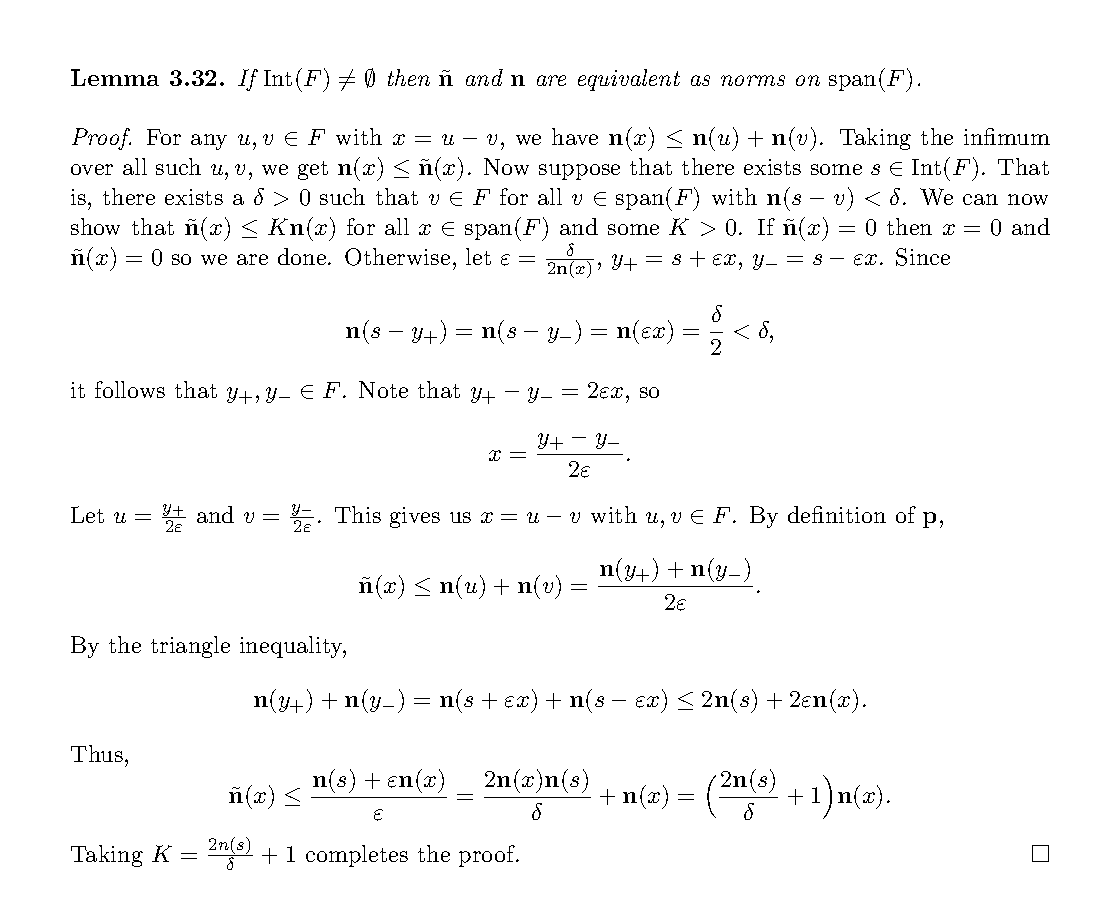
\includegraphics[width=0.94\linewidth]{figures/interior_lemma_crop.png}
\caption{The source's positive result under nonempty interior, printed page 22.}
\end{figure}

\section{Verification and novelty status}

The construction was audited directly in the source's conventions: $F$ is a
cancellative cone, its canonical span is identified with $V$, and
\eqref{eq:extension} is exactly the source's extension norm.  The lower bound
uses only uniqueness of finite basis expansions and two standard-coordinate
projections.  No limiting point outside $c_{00}$ is invoked in the proof of
closedness, which is relative to the stated normed space.

Bounded exact-phrase, title, generating-cone, bounded-decomposition, and
And\^o-theorem searches found the source question and the classical positive
theory, but no later paper explicitly answering this particular question or
this block-basis counterexample.  The underlying phenomenon is standard in
ordered normed-space theory, so novelty is claimed only for the explicit
answer and its connection to arXiv:2508.17052.  Expert or author review is
recommended before dissemination.

\begin{thebibliography}{9}
\bibitem{KO}
E. Kharitonov and A. Ohanyan,
\emph{Topological cones and positively polarizable hyperbolic norms},
arXiv:2508.17052 (2025), Proposition 2.20, Lemma 2.22, and Lemma 3.32.

\bibitem{Ando}
T. And\^o,
\emph{On fundamental properties of a Banach space with a cone},
Pacific J. Math. \textbf{12} (1962), 1163--1169,
\href{https://doi.org/10.2140/pjm.1962.12.1163}{doi:10.2140/pjm.1962.12.1163}.
\end{thebibliography}

\end{document}
